\documentclass[11pt, spanish]{article}
\usepackage[utf8]{inputenc}
\usepackage{listings} 
\usepackage{graphicx}
\usepackage{amsfonts}
\usepackage[dvipsnames]{xcolor}
\usepackage[T1]{fontenc}
\usepackage{bigfoot}
\usepackage{amsmath}
\usepackage{algorithm}
\usepackage[noend]{algpseudocode}
\usepackage[numbered,framed]{matlab-prettifier}
\usepackage{caption}
\usepackage{blkarray}
\usepackage{float}
\usepackage{xcolor}
\usepackage{multicol}
\usepackage[rightcaption]{sidecap}

\makeatletter
\def\@seccntformat#1{%
  \expandafter\ifx\csname c@#1\endcsname\c@section\else
  \csname the#1\endcsname\quad
  \fi}
\makeatother

\makeatletter
\def\BState{\State\hskip-\ALG@thistlm}
\makeatother

\makeatletter
    \setlength\@fptop{0\p@}
\makeatother

\date{}

\usepackage{geometry}
 \geometry{
 a4paper,
 left=30mm,
 right=30mm,
 top=30mm,
 }

\lstset{
	style              = Matlab-editor,
  	basicstyle         = \mlttfamily,
  	escapechar         = ",
  	mlshowsectionrules = true,
	framesep=4.5mm,
	framexleftmargin=2.5mm,
	fillcolor=\color{White},
	rulecolor=\color{Black},
	numberstyle=\normalfont\tiny\color{Black}
}

\captionsetup[lstlisting]{font={small,tt}}
\renewcommand{\lstlistingname}{Script}
\newcommand\RED{\color{red}}
\newcommand\BLUE{\color{blue}}
\newcommand{\BigO}[1]{\ensuremath{\operatorname{O}\bigl(#1\bigr)}}
\newcommand{\norm}[1]{\left\lVert#1\right\rVert}
\newcommand{\divides}{\bigm|}
\renewcommand{\figurename}{Figura.}
\newcommand{\ndivides}{%
  \mathrel{\mkern.5mu % small adjustment
    % superimpose \nmid to \big|
    \ooalign{\hidewidth$\big|$\hidewidth\cr$\nmid$\cr}%
  }%
}

\begin{document}

\renewcommand\lstlistlistingname{Lista de Scripts}

\author{Sebastián Valencia Calderón \\ 201111578}
\title{Tarea 2: Método de Bairstow y factorización de Cholesky}
\maketitle

%====================================================================

\section{Proyecto 1}

Ciertas propiedades de una matriz $A \in \mathbb{R}$, pueden ser usadas para mejorar la eficiencia del método de eliminación de Gauss para resolver un sistema del tipo $Ax = b$. En particular, si $A \in \mathbb{R}^{n \times n}$ es una matriz simétrica y positiva definida, el trabajo computacional se reduce a la mitad, lo que representa una mejora de eficiencia dramática. El objetivo de este proyecto, es el de explorar la naturaleza de un algoritmo que explota ambas propiedades de una matriz: que sea simétrica y positiva definida. a continuación, se definen las matrices a usar: una matriz $A \in \mathbb{R}^{n \times n}$ es simétrica si $a_{ij} = a_{ji}\ \forall\ i,\ j\ \in \{1,\ 2,\ \dots,\ n\}$, es decir $A = A^T$. El conjunto de todas las matrices simétricas es $\mathbb{R}_{\text{sym}}^{n \times n}$. Una matriz es positiva definida si $x^TAx > 0$ para todo vector $x \in \mathbb{R}^n \setminus \{ 0\}$. Las matrices positivas definidas, poseen ciertas características que se pueden explotar para resolver sistemas lineales donde ellas estén involucradas. En particular, si $n \geq 2$ y $A \in \mathbb{R}_{\text{sym}}^{n \times n}$, entonces:

\begin{itemize}
\item Todos los elementos de la diagonal son positivos.

\item Todos los valores propios de A son reales y positivos.

\item El determinante de $A$ es positivo.

\item $a_{ij}^2 < a_{ii}a_{jj}\ \forall\ i,\ j\ \in \{1,\ 2,\ \dots,\ n\} \wedge i \neq j$.
\end{itemize}

Una matriz simétrica, tiene un conjunto ortonormal de vectores propios, cada uno distinto de cero, además, los valores propios correspondientes son todos reales, por lo que un vector $x \in \mathbb{R}^{n} \setminus \{ 0 \}$, puede expresarse como una combinación lineal de los vectores propios de $A$. Si $A$ es simétrica y positiva definida, se puede obtener una factorización $A=LU$, donde $U = L^T$. (estas propiedades, pueden estudiarse más a fondo en la referencia \cite{suli2003introduction}) La deducción del algoritmo, está incluida en las referencias: . Por motivos prácticos, se incluye una generalización del mismo a partir del cálculo de la factorización para una matriz $A \in \mathbb{R}^{4 \times 4}$.

\[
\begin{bmatrix}
    a_{11} & a_{12} & a_{13} & a_{14} \\
    a_{21} & a_{22} & a_{23} & a_{24} \\
    a_{31} & a_{32} & a_{33} & a_{34} \\
    a_{41} & a_{42} & a_{43} & a_{44} 
\end{bmatrix}
=
\begin{bmatrix}
    u_{11} & 0 & 0 & 0 \\
    u_{21} & u_{22} & 0 & 0 \\
    u_{31} & u_{32} & u_{33} & 0 \\
    u_{41} & u_{42} & u_{43} & u_{44} 
\end{bmatrix}
\times
\begin{bmatrix}
    u_{11} & u_{12} & u_{13} & u_{14} \\
    0 & u_{22} & u_{23} & u_{24} \\
    0 & 0 & u_{33} & u_{34} \\
    0 & 0 & 0 & u_{44} 
\end{bmatrix}
\]\\
\[
=\begin{bmatrix}

    u_{11}^2 & 
    u_{11}u_{12} & 
    u_{11}u_{13} & 
    u_{11}u_{14} \\
    
    u_{12}u_{11} & 
    u_{12}^2+u_{22}^2 & 
    u_{12}u_{13}+u_{22}u_{23} & 
    u_{12}u_{14}+u_{22}u_{24} \\
    
    u_{13}u_{11} & 
    u_{13}u_{12}+u_{23}u_{22} & 
    u_{13}^2+u_{23}^3+u_{33}^2 &
    u_{13}u_{14}+u_{23}u_{24}+u_{33}u_{34} \\
    
    u_{13}u_{11} & 
    u_{14}u_{12}+u_{24}u_{22} & 
    u_{14}u_{13}+u_{24}u_{23}+u_{34}u_{33} & 
    u_{14}^2+u_{24}^2+u_{34}^2+u_{44}^2
    
\end{bmatrix}
\]
        
\begin{itemize}
\item \textbf{Algoritmo.} Cálculos algebraicos basados en la igualdad de matrices y la multiplicación matricial, y en los cálculos realizados para la matriz de dimensión $4 \times 4$ (ilustración original en la referencia \cite{yang2005applied}), sugieren lo siguiente:

$$u_{kk} = \sqrt{a_{kk} - \sum_{i = 1}^{k - 1}(u_{ik}^2)} \quad u_{km} = \frac{\left[ a_{km} - \sum_{i = 1}^{k-1} \left( u_{im}u_{ik}\right)\right]}{u_{kk}} \quad \begin{cases} 
      k \in \{1,\dots, N\} \\
      m \in \{k+1,\dots, N\} 
   \end{cases}$$
   
Una primera aproximación sencilla al algoritmo dadas las fórmulas obtenidas por medio de la generalización, se muestra a continuación:

\begin{algorithm}[h]
\caption{Cholesky factorization based on formulas above}
\label{alg:choleskynaive}
\begin{algorithmic}[1]
\Require $A \in \mathbb{R}_{\text{sym}}^{n \times n} \wedge A \text{ is positive definite}$
\Ensure $L \text{ is lower triangular} \wedge L^TL = A$
\Procedure{Cholesky}{}
\State $L \in \mathbb{R}^{n \times n}$
\For{$k \gets 1\ \dots\ n$}
\State $L_{kk} \gets \sqrt{a_{kk} - \sum_{s = 1}^{k - 1}(l_{ks}^2)}$
\For{$i \gets (k+1)\ \dots\ n$}
\State $L_{ik} \gets  \frac{\left[ a_{ik} - \sum_{s = 1}^{k-1} \left( u_{is}u_{ks}\right)\right]}{l_{kk}}$
\EndFor
\EndFor
\Return{$L$}
\EndProcedure
\end{algorithmic}
\end{algorithm}

Para aproximar el algoritmo \ref{alg:choleskynaive}, a una implementación sobre una máquina digital usando un lenguaje de programación real, se puede reescribir de esta forma (considerando error en la forma de la matriz).

\begin{algorithm}[h]
\caption{Cholesky factorization for real implementation}
\label{alg:choleskyreal}
\begin{algorithmic}[1]
\Require $A \in \mathbb{R}^{n \times n}$
\Ensure $L \text{ is lower triangular} \wedge L^TL = A \text{ iff } A \text{ is positive definite.}$
\Procedure{Cholesky}{}
\For{$i \gets 1\ \dots\ n$}
\State $t \gets a_{ii} - \sum_{j = 1}^{i - 1}l_{ji}^2$
\If{$t \leq 0$}
\State $A \text{ is not positive definite }$
\Return{$error$}
\EndIf
\State $l_{ii} \gets \sqrt{t}$
\For{$j \gets (i + 1)\ \dots\ n$}
\State $l_{ij} \gets \frac{a_{ij} - \sum_{k=1}^{i-1}l_{ki}l_{kj}}{l_{ii}}$
\EndFor
\EndFor
\Return{$L$}
\EndProcedure
\end{algorithmic}
\end{algorithm}

El último algoritmo, puede representarse fácilmente en un lenguaje de programación como \textsc{Matlab}, basta con representar las sumatorias como productos puntos y ya está. El manejo de error, también hace propicio la implementación del algoritmo \ref{alg:choleskyreal}, en el lenguaje de programación, además, constituye una buena prueba para verificar si una matriz es positiva definida. A continuación, se incluye el código implementado en \textsc{Matlab}, y la validación del mismo mediante el uso de algunas matrices de dimensión variable.

\item \textbf{Implementación.} La implementación del algoritmo \ref{alg:choleskynaive}, en una máquina digital por medio de un lenguaje de programación de alto nivel como \textsc{Matlab}, requiere contemplar la verificación de la positividad de la matriz $A$. Esta verificación, surge de manera natural con el diseño del algoritmo \ref{alg:choleskyreal}, el cual materializa la verificación, por medio de una sencilla manipulación a las fórmulas derivadas anteriormente. La única función pues necesaria para la realización de la factorización de Cholesky de una matriz es la siguiente:

\lstinputlisting[caption = {Factorizacion de Cholesky, desarrollo del algoritmo \ref{alg:choleskyreal}.}, label={lst:cholesky}]{data/scripts/cholesky.m}

\newpage

\item \textbf{Validación.} Para validar la implementación, se propone además de lo pedido, tomar ejemplos disponibles en la bibliografía (es enspecífico, las referencias \cite{cheney2007numerical}, \cite{watkins2004fundamentals}, y \cite{ford2014numerical}), comparar el resultado expuesta en la misma con la ejecución de la factorización programada. A continuación, se muestra un ejemplo de dicha factorización presente en la referencia \cite{watkins2004fundamentals}, además, se contrasta esto con la ejecución del código escrito sobre la representación de la misma matriz.

Ejemplo:

$$A = \begin{bmatrix}
    4 & -2 & 4 & 2\\ -2 & 10 & -2 & -7\\ 4 & -2 & 8 & 4\\ 2 & -7 & 4 & 7 
\end{bmatrix} \Rightarrow L = \begin{bmatrix} 2 & -1 & 2 & 1\\ 0 & 3 & 0 & -2\\ 0 & 0 & 2 & 1\\ 0 & 0 & 0 & 1 \end{bmatrix}$$

Le ejecución de estas lineas:\\

\lstinputlisting[caption = {}, label={lst:examplechol}]{data/scripts/examplechol.m}

Da como resultado:

$$L = \begin{bmatrix} 2 & -1 & 2 & 1\\ 0 & 3 & 0 & -2\\ 0 & 0 & 2 & 1\\ 0 & 0 & 0 & 1 \end{bmatrix}
$$

Ahora, se valida haciendo uso de una matriz tridiagonal con valor 4 en la diagonal principal, y -1 en las diagonales adyacentes. Con esta descripción, se generan matrices de tamaño 10, 20 y 30, se calcula la factorización de Cholesky con el método implementado \texttt{cholesky}, y con la función de \textsc{Matlab} \texttt{chol}, se comparan ambos resultados ($\norm{L^T \times T -A}_\infty$) a partir de su efectividad. Para esto, se tiene el siguiente script que genera la matriz según su tamaño:\\

\lstinputlisting[caption = {}, label={lst:genmatrix}]{data/scripts/genmatrix.m}\

Por ejemplo, \texttt{genmatrix(5)} da como resultado:\

$$A = \begin{bmatrix}
    4 & -1 & 0 & 0 & 0\\ -1 & 4 & -1 & 0 & 0\\ 0 & -1 & 4 & -1 & 0\\ 0 & 0 & -1 & 4 & -1\\ 0 & 0 & 0 & -1 & 4 
\end{bmatrix}$$

Ahora, se ejecuta el siguiente script para validar la ejecución de la función implementada y contrastar sus resultados con los de la librería estándar de \textsc{Matlab}. De esta manera, se obtiene una comparación entre el comportamiento y desempeño numérico de ambas funciones.\\

\lstinputlisting[caption = {}, label={lst:validatechol}]{data/scripts/validatechol.m}\

Al graficar los resultados obtenidos con el anterior script, se obtiene lo siguiente:

\begin{figure}[h]
    \centering
    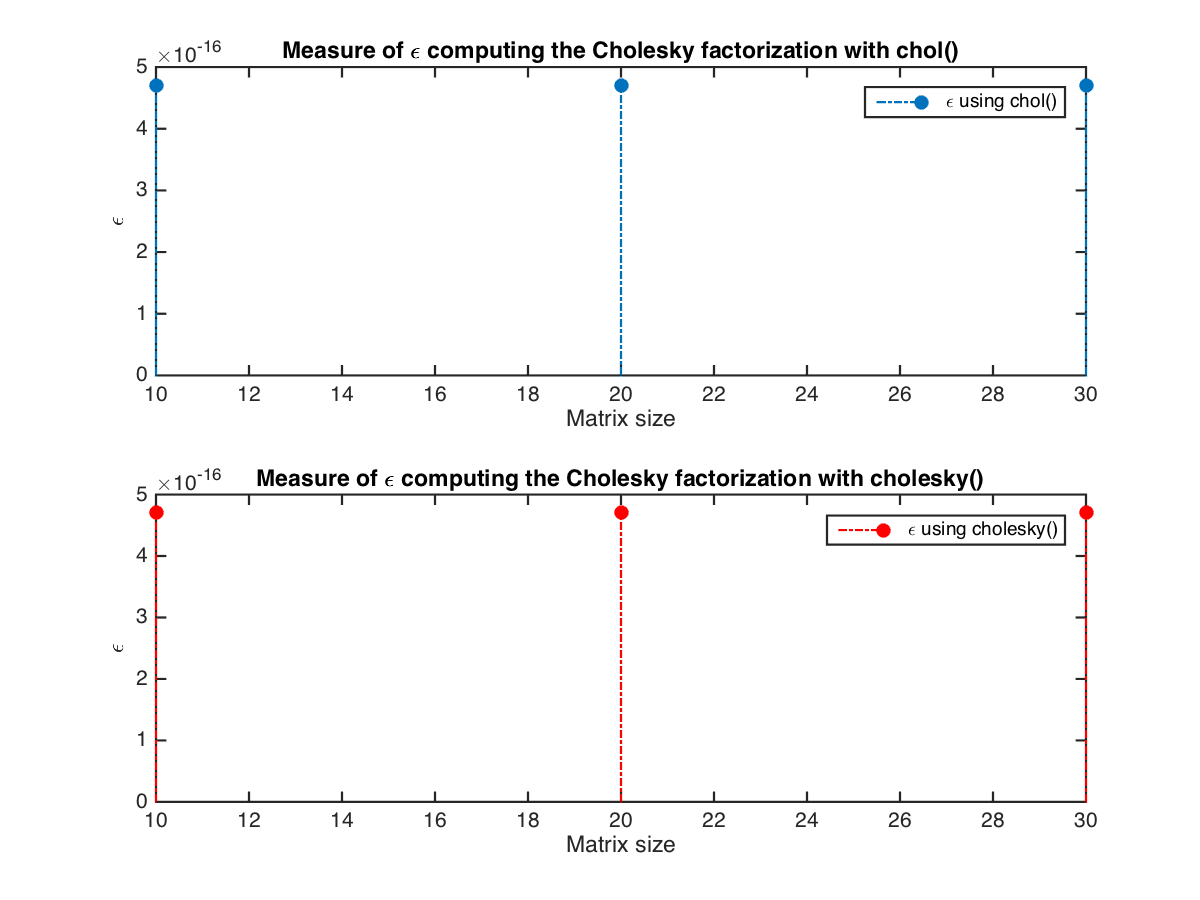
\includegraphics[width=14cm]{data/img/cholcomparisson}
    \caption{Comparación de las dos funciones para factorizar una matriz positiva definida, la métrica de error, está dada por la expresión $\norm{L^T \times L - A}$. El desempeño y comportamiento de ambas funciones es el mismo.}
    \label{fig:cholcomparisson}
\end{figure}

\end{itemize}

%==================================================================

\newpage
\section{Proyecto 2}

Un polinomio, es una estructura algebraica o ecuación de la forma:

$$P_{n}(x)\ :\ a_{0}x^{n} + a_{1}x^{n-1} + a_{2}x^{n-2} + \dots + a_{k}x^{n-k} + \dots + a_{n-1}x  + a_{n} = 0 $$\

Donde los coeficientes $a_i$, son números específicos en $\mathbb{Z}$, $\mathbb{Q}$, $\mathbb{R}$, o $\mathbb{C}$. Para resolver este tipo de ecuaciones, es necesario hallar otro número puntual $x$ que satisfaga la ecuación. Es decir, dado un polinomio $P_{n}(x)$, solucionar el polinomio, es encontrar el conjunto $X$:

$$X = \{ x \in \mathbb{C}\ |\ P_{n}(x) = 0\}$$\

El número $n$, es denominado orden del polinomio, este determina la cardinalidad de $X$, de manera más específica, $n$, o $|X|$, es el número de raíces del polinomio, es decir, cada uno de los elementos pertenecientes a $X$, los cuales, por definición satisfacen $P_n(X) = 0$. Conocer de antemano la cantidad de raíces de un polinomio, es un hecho matemático de fundamental importancia para la solución computacional del polinomio. Otra deducción matemática fundamental para esta tarea, es el teorema fundamental del álgebra, el cual, se presta para deducir que si un numero complejo $a + ib$ pertenece a $X$, entonces el numero complejo $a - ib$, también lo hace.\\

Los polinomios, son una estructura fundamental en la computación científica, al igual que las matrices, muchos problemas de computación científica, pueden reducirse a ecuaciones no lineales polinomiales. Por esta razón, es importante el diseño de algoritmos numéricos para la solución de este tipo de ecuaciones. Si $n \leq 3$, el problema es trivial, en el caso de $n = 1$, el problema se resuelve con dos multiplicaciones y una división. Si $n = 2$, existe la famosa fórmula para hallar las dos raíces. Si $n = 3$ , se puede recurrir a las fórmulas de Cardano. Para grados mayores a 3, existe una dificultad inherente a las estructuras matemáticas comprometidas en la solución y estructura de los polinomios (los artilugios del álgebra abstracta). Para mitigar esto, se presenta un método para la solución numérica de un polinomio $P_n(x)$. A continuación, se presenta un método para la solución no analítica de un polinomio (La exposición referida, es presentada de manera formal en la referencia \cite{rosloniec2008fundamental}. Una derivación alternativa y más cercana al cálculo matricial, es presentada en la referencia \cite{miller2014numerical}).\\

Un polinomio de la forma $P_n(x) = \sum_{i = 0}^{n} a_ix^{n - i}$, ($a_0 = 1$), puede escribirse se la forma:

$$(x^2+px+q)(x^{n - 2} + b_{1}x^{n - 3} + b_{2}x^{n-4} + \dots + b_{k}x^{n-2-k} + \dots b_{n-3}x + b_{n-2}) + Rx + S = 0$$

En la anterior expresión, $Rx + S$, es el residuo lineal, el cual, se debe iterativamente reducir para lograr una igualdad entre esta última expresión y el polinomio original. En este caso, el polinomio original $P_n(x)$, es divisible perfectamente con $(x^2+px+q)$. La manipulación algebraica, es suficiente para relacionar los coeficientes $p,\ q,\ b1,\ b2,\ b_3,\ \dots,\ b_{n-2}$, $R$, y $S$ con los coeficientes del polinomio normalizado (aquel polinomio donde $a_0 = 1$) . A continuación, se muestra la relación:

\begin{eqnarray*}
b_{1} & = & a_{1} - p \\
b_{2} & = & a_{2} - p b_{1} - q \\
b_{i} & = & a_{i} - p b_{i - 1} - qb_{i - 2}\ \ \ i = 1 \dots (n - 2) \\
R & = & a_{n-1} - p b_{n-2} - qb_{n-3} \\
S & = & a_{n} - qb_{n - 2}
\end{eqnarray*}

Si $R = 0\ \wedge\ S = 0$, las raíces del término cuadrático $(x^2+px+q)$, son también raíces del polinomio original $P_n(x)$. Estas raíces, son fácilmente obtenidas mediante el uso de la fórmula cuadrática. Ahora, es necesario hallar coeficientes $p,\ q,\ b1,\ b2,\ b_3,\ \dots,\ b_{n-2}$ para satisfacer la proposición $R = 0\ \wedge\ S = 0$, de esta manera, a partir de la expresión cuadrática obtenida, se pueden hallar dos raíces de $P_n(x)$. El polinomio, en la reducción de los términos hasta lograr $R = 0\ \wedge\ S = 0$, queda agrupado así $P_n(x) = (x^2+px+q)P_{n-2}(x)$. Es necesario, reducir ahora $P_{n-2}(x)$ de la misma forma hasta lograr que el polinomio que acompaña el término cuadrático sea fácil de resolver (usando la fórmula de Cardano o la fórmula cuadrática).\\

El método de Bairstow, usa aproximaciones de $p$ y de $q$ haciendo uso del método de Newton:

\begin{eqnarray*}
p^{(n + 1)} & = & p^{(n)} - \frac{\left( R \times \frac{\partial S}{\partial q} - S \times \frac{\partial R}{\partial q}\right)}{J}\\
q^{(n + 1)} & = & q^{(n)} + \frac{\left( R \times \frac{\partial S}{\partial p} - S \times \frac{\partial R}{\partial p}\right)}{J} \\
\textbf{Donde}\ J & = & \left[\frac{\partial R}{\partial p} \frac{\partial S}{\partial q} - \frac{\partial S}{\partial p} \frac{\partial R}{\partial q}\right]
\end{eqnarray*}\

Dado que $R$ y $S$ son funciones de $b1,\ b2,\ b_3,\ \dots,\ b_{n-2}$, los cuales a su vez dependen de $p$ y de $q$, es necesario hallar las derivaras parciales respecto a $p$ y a $q$ de los coeficientes $b1,\ b2,\ b_3,\ \dots,\ b_{n-2}$, $R$, y $S$. A continuación, se halla cada derivada parcial:

\begin{eqnarray*}
\nabla b_{1}(p, q) & = & \left[ c_1, d_1 \right] = \left[ -1, 0 \right] \\
\nabla b_{2}(p, q) & = & \left[ c_2, d_2 \right] = \left[ -b_1 - p \left( \frac{\partial b_1}{\partial p}\right),  - p \left( \frac{\partial b_1}{\partial q}\right) - 1 \right] =  \left[ -b_1 + p, -1 \right]\\
\nabla b_{i}(p, q) & = & \left[ c_i, d_i \right] = \left[ -b_{i-1} - p \left( \frac{\partial b_{i-1}}{\partial p}\right) - q \left( \frac{\partial b_{i-2}}{\partial p}\right) ,  - p \left( \frac{\partial b_{i-1}}{\partial q}\right) - b_{i-2} - q \left( \frac{\partial b_{i-2}}{\partial q}\right) \right] \\
& = &\left[ -b_1 + p, -1 \right]\ \ \ i = 3 \dots (n - 2) \\
\end{eqnarray*}

\begin{eqnarray*}
\nabla R(p, q) & = & \left[ -b_{n-2} - p \left( \frac{\partial b_{n-2}}{\partial p} \right) - q \left( \frac{\partial b_{n-3}}{\partial p} \right),  -p \left( \frac{\partial b_{n-2}}{\partial q}\right) -b_{n-3}  - q \left( \frac{\partial b_{n-3}}{\partial q} \right)\right] \\
\nabla S(p, q) & = & \left[- q \left( \frac{\partial b_{n-2}}{\partial p} \right) , -b_{n-2}  - q \left( \frac{\partial b_{n-2}}{\partial q} \right)\right] 
\end{eqnarray*}

Haciendo uso de los coeficientes $c_i$ y $d_i$, es posible reescribir los términos $\nabla R(p, q)$, $\nabla S(p, q)$,  $\nabla b_{i = 1 \dots (n - 2)}(p, q)$ de la siguiente manera:

\begin{eqnarray*}
\nabla b_{1}(p, q) & = & \left[ c_1, d_1 \right] = \left[ -1, 0 \right] \\
\nabla b_{2}(p, q) & = & \left[ c_2, d_2 \right] =  \left[ -b_1 + p, -1 \right]\\
\nabla b_{i}(p, q) & = & \left[ c_i, d_i \right] = \left[ -b_{i-1} - p c_{i-1} - q c_{i-2}, -b_{i-2} - p d_{i-1} - q d_{i-2} \right]\ \ \ i = 3 \dots (n - 2) \\
\nabla R(p, q) & = & \left[-b_{n-2} - p c_{n-2} - qc_{n-3}, -b_{n-3} - pd_{n-2}-qd_{n-3}\right] \\
\nabla S(p, q) & = & \left[-qc_{n-2}, -b_{n-2}-q d_{n-2}\right]
\end{eqnarray*}

Las formulas escritas anteriormente, aplican para ecuaciones polinomiales de grados estrictamente mayores a 3. Para ecuaciones de grados menores, se recurre a la solución trivial.

\begin{algorithm}[h]
\caption{}
\label{alg:bairstow}
\begin{algorithmic}[1]
\Require $n \geq 4\ \wedge\ P_n(x) : \sum_{i = 0}^{n} a_ix^{n - i}\ ,\ a_0 = 1$
\Ensure $P_n(x) = (x^2 + px + q)(x^{n - 2} + b_{1}x^{n - 3}  + \dots + b_{k}x^{n-2-k} + \dots b_{n-3}x + b_{n-2})$
\Procedure{Bairstow}{}
\State $p,\ q \gets 0,\ 0$
\State $n \gets \text{Degree of } P_n(x)$
\State $R,\ S \gets \infty,\ \infty$
\State $b,\ c,\ d \text{ : Are polynomials of degree } (n - 2)$
\While{$\epsilon < |R + S|$}
\State $b_1,\ b_2 \gets a_{1} - p,\ a_{2} - p b_{1} - q$
\State $c_1,\ c_2 \gets -1,\ -b_1 + p$
\State $d_1,\ d_2 \gets 0, -1$
\For{$i \in \{ 3,\ \dots\ ,\ n - 2\}$}
\State $b_i \gets a_{i} - p b_{i - 1} - qb_{i - 2}$
\State $c_i,\ d_i \gets  -b_{i-1} - p c_{i-1} - q c_{i-2}, -b_{i-2} - p d_{i-1} - q d_{i-2}$
\EndFor
\State $R,\ S \gets a_{1} - p,\ a_{2} - p b_{1} - q$
\State $\nabla R(p, q) \gets \left[-b_{n-2} - p c_{n-2} - qc_{n-3},\ -b_{n-3} - pd_{n-2}-qd_{n-3}\right]$
\State $\nabla S(p, q) \gets \left[-qc_{n-2},\ -b_{n-2}-q d_{n-2}\right]$
\State $J \gets \left[\frac{\partial R}{\partial p} \frac{\partial S}{\partial q} - \frac{\partial S}{\partial p} \frac{\partial R}{\partial q}\right]$
\State $p,\ q \gets p - \frac{\left( R \times \frac{\partial S}{\partial q} - S \times \frac{\partial R}{\partial q}\right)}{J},\ q + \frac{\left( R \times \frac{\partial S}{\partial p} - S \times \frac{\partial R}{\partial p}\right)}{J}$
\EndWhile
\Return{$p,\ q,\ x^{n - 2} + b_{1}x^{n - 3} + b_{2}x^{n-4} + \dots + b_{k}x^{n-2-k} + \dots b_{n-3}x + b_{n-2}$}
\EndProcedure
\end{algorithmic}
\end{algorithm}

\begin{itemize}
\item \textbf{Algoritmo.} El aparato teórico expuesto anteriormente, permite plantear un algoritmo para hallar la factorización de un polinomio $P_n(x)$ donde $n \geq 4$. Es decir, pado un polinomio $P_n(x)$, se pretende diseñar un algoritmo que calcule $p$, $q$, términos necesarios para el término cuadrático, y $b_i$, que garanticen que $R$ y $S$, se encuentren en un radio muy pequeño cuyo centro es cero. El algoritmo de Bairstow, es usado para hallar la factorización cuadrática de un polinomio $P_n(x)$. Dicha factorización es: $(x^2+px+q)(x^{n - 2} + b_{1}x^{n - 3} + b_{2}x^{n-4} + \dots + b_{k}x^{n-2-k} + \dots b_{n-3}x + b_{n-2}) + Rx + S$, tal que $R$ y $S$ sean tan pequeños como se requiera (computacionalmente hablando), dependiendo de un error $\epsilon$.\\

El algoritmo \ref{alg:bairstow}, asigna los valores pertinentes (los cuales fueron deducidos anteriormente) a los coeficientes $b_1,\ b_2,\ \dots\ ,\ b_i$, y finalmente a $p$ y a $q$ según las igualdades expuestas en la deducción matemática. Este proceso, se repite hasta que $\epsilon \geq |R + S|$. Cuando esto se cumpla, se cuenta con valores de $p$, $q$, $b_i$, para formar la expresión $(x^2 + px + q)(x^{n - 2} + b_{1}x^{n - 3}  + \dots + b_{k}x^{n-2-k} + \dots b_{n-3}x + b_{n-2})$, que sea igual a $P_n(x)$. Con esta factorización, se obtienen las dos primeras raíces del polinomio original $P_n(x)$:

$$x^{(1)} = \frac{-p + \sqrt{p^2 - 4q}}{2} \qquad  x^{(2)} = \frac{-p - \sqrt{p^2 - 4q}}{2}$$

Se puede aplicar de nuevo el algoritmo \ref{alg:bairstow}, sobre el polinomio $x^{n - 2} + b_{1}x^{n - 3}  + \dots + b_{k}x^{n-2-k} + \dots b_{n-3}x + b_{n-2}$, para obtener las raíces $x^{(3)}$, y $x^{(4)}$, así, de manera sucesiva, se obtienen raíces hasta que la expresión $x^{n - 2} + b_{1}x^{n - 3}  + \dots + b_{k}x^{n-2-k} + \dots b_{n-3}x + b_{n-2}$, tenga un grado menor a 4. En cuyo caso, se debe aplicar el método trivial. Esta aplicación repetida del algoritmo \ref{alg:bairstow}, sugiere el siguiente procedimiento para hallar todas las raíces de un polinomio.

\begin{algorithm}[h]
\caption{}
\label{alg:roots}
\begin{algorithmic}[1]
\Require $P_n(x) : \sum_{i = 0}^{n} a_ix^{n - i}\ ,\ a_0 \neq 0 $
\Ensure $X = \{ x \in \mathbb{C}\ |\ P_{n}(x) = 0\}$
\Procedure{PolynomialRoots}{}
\State $n \gets \text{Degree of } P_n(x)$
\State $X \gets \{ \}$
\If{$n \leq 3$}
\State Solve it using algebraic methods (quadratic formula, Cardano's method).
\State Direct algebraic solution.
\State $X\gets X \cup \textsc{Solve}(P_n(x))$
\Else
\State $ P_n(x) \gets \sum_{i = 0}^{n} \left(\frac{a_i}{a_0}\right)x^{n - i}$
\While{$n > 3$}
\State $p,\ q,\ P_n(x) \gets \textsc{Bairstow}(P_n(x),\ \epsilon)$
\State $X \gets X \cup \textsc{Solve}(x^2+px+q)$
\State $n \gets \text{Degree of } P_n(x)$
\EndWhile
\State $X\gets X \cup \textsc{Solve}(P_n(x))$
\EndIf
\Return{$X$}
\EndProcedure
\end{algorithmic}
\end{algorithm}

El algoritmo \ref{alg:roots}, dependiendo del grado del polinomio, resuelve este de manera algebraica o de manera numérica. Si $n \leq 3$, entonces lo hace de la primera forma (aplicando la fórmula cuadrática o la fórmula de Cardano), de lo contrario, normaliza el polinomio (linea 9 del algoritmo \ref{alg:roots}), de tal forma que $a_0 = 1$. Posteriormente, se aplica iterativamente (reduciendo el grado a $i - 2$ por cada iteración) el método de Bairstow (algoritmo \ref{alg:bairstow}), para obtener la factorización de cada polinomio. La linea 11 de este algoritmo \ref{alg:roots}, calcula $p$, $q$, y el nuevo valor del polinomio. Con los dos primeros términos ($p$ y $q$), se hallan dos raíces más del polinomio original (haciendo uso de la formula cuadrática), y finalmente, se agregan al conjunto de solución $X$. Después del proceso iterativo, por un hecho expuesto más adelante, se cuenta con un polinomio de grado menor a 4, por lo que las raíces de este, se calculan de manera algebraica, a través de la función \textsc{Solve}, el cual para polinomios de grado 1 debe despejar $x$, para polinomios de grado 2 debe calcular $X$ haciendo uso de la fórmula cuadrática, y para polinomios cúbicos, debe usar el método de Cardano. Esta sugerencia, se adopta de la referencia \cite{rosloniec2008fundamental}.\\

\textbf{Definición:} Sea $\mathbb{N}_e = \{n \in \mathbb{N}^+\ |\ \exists\ k \in \mathbb{N}^+\ ;\ n = 2 k\}$, sea $\mathbb{N}_o = \mathbb{N}^+ \setminus \mathbb{N}_e  $.\\

Dado $P_n(x)$, si $n$ es par, $n \in \mathbb{N}_e $. Por el lema de Zorn, se sabe que $n$ está contenido en un conjunto $E = \{2,\ 4,\ \dots ,\ n,\ 2(n + 1) \}$. De manera equivalente, si $n \in \mathbb{N}_o$, $\exists\ O \subset \mathbb{N}_o$ tal que $O = \{1,\ 3,\ \dots ,\ n,\ 2n + 1 \}$. Sea $pred_A$ una función con tipo $pred\ :\ A \setminus \{ \min{A}\} \rightarrow A$, que para cada elemento en $A \setminus 	\{ \min{A}\}$, retorne el predecesor absoluto bajo una ordenación isomorfa a la $\mathbb{N}$. Es decir, $pred_E\ :\ E \setminus \{ 2\} \rightarrow E $, retorna el par anterior a $n$. Una construcción análoga para los números impares, permite deducir que la aplicación finita y sucesiva de $pred$ a algún $n$ sobre el conjunto al cual pertenezca ($E$, u $O$), terminara en 2 o en 3, dependiendo si $n$ es par o impar respectivamente.\\

La anterior deducción, aunque un tanto formal, es útil para demostrar que al salir del loop de la linea 10 del algoritmo \ref{alg:roots}, $P_n(x)$, sera tal que $n \leq 3$, la aplicación sucesiva descendiente de $pred$, mas que la condición de parada, sirven para demostrar la terminación del algoritmo en cuestión. Suponiendo que el algoritmo \ref{alg:bairstow}, termina, se ha diseñado un algoritmo capaz de hallar con cierto error o tolerancia, las raíces de un polinomio de grado arbitrario.

\item \textbf{Implementación.} La implementación del algoritmo \ref{alg:roots}, en una máquina digital por medio de un lenguaje de programación de alto nivel como \textsc{Matlab}, requiere contemplar el desarrollo de la formula cuadrática y del método de Cardano para la solución algebraica de polinomios de grados que así lo permitan (Galois y Abel). A continuación, se muestran documentados los archivos de \textsc{Matlab}, que permiten la materialización del algoritmo \ref{alg:roots}, se muestran, de orden de relevancia, es decir, se muestra de ultimo el algoritmo final, antes de este, se muestran las funciones necesarias para su realización.

\lstinputlisting[caption = {Obtención de raíces de un caso trivial: un polinomio cuadrático.}, label={lst:quadratic}]{data/scripts/quadratic.m}

\lstinputlisting[caption = {Fórmulas de Cardano para la transformación y posterior solución de ecuaciones de tercer grado.}, label={lst:cardano}]{data/scripts/cardano.m}

\lstinputlisting[caption = {Obtención de la solución algebraica, dependiendo el orden o grado del polinomio dado como parámetro. Esta función únicamente resuelve el polinomio si $n \leq 3$.}, label={lst:basecase}]{data/scripts/basecase.m}

\lstinputlisting[caption = {Obtención de una versión equivalente a un polinomio, pero con el coeficiente que define el grado, puesto en 1.}, label={lst:normalized}]{data/scripts/normalized.m}

\newpage

\lstinputlisting[caption = {Algoritmo de Bairstow para calcular la factorización cuadrática de un polinomio de grado mayor a 3. Es una implementación del algoritmo 	\ref{alg:bairstow}. El término cuadrático de la factorización, determina dos de las raíces del polinomio dado por parámetro.}, label={lst:bairstow}]{data/scripts/bairstow.m}

\lstinputlisting[caption = {Solución de ecuaciones de grado arbitrario mediante el uso (de ser posible), de manipulación algebraica, en otro caso, de una secuencia de aplicaciones del algoritmo \ref{alg:bairstow} sobre el polinomio y su residuo. Es una implementación de \ref{alg:roots}.}, label={lst:nroots}]{data/scripts/nroots.m}

\item \textbf{Validación.} Como primer medida de validación, se pueden tomar los ejemplos de los textos citados (\cite{rosloniec2008fundamental}, \cite{miller2014numerical}). A continuación, se muestran dos polinomios con sus raíces respectivas (según los textos), además, se muestra la ejecución del código escrito sobre la representación de los mismos polinomios:

Ejemplo tomado de la referencia \cite{miller2014numerical}:

$$P_6(x) : 5x^6 - 30x^5 +56x^4 - 96x^3 + 131x^2-18x+24 = 0$$
$$R = \{ 5.3091 \times 10^{-18} \pm 0.44721j,\ 4.7003 X 10^{-17} \pm 1.7321j,\ 4,\  2\}$$

La ejecución de estas lineas:

\lstinputlisting[caption = {}, label={lst:example1}]{data/scripts/example1.m}

Da como resultado:

\texttt{rs = [0.0000 + 0.4472i   \qquad 0.0000 - 0.4472i  \qquad -0.0000 + 1.7321i} \\
\texttt{-0.0000 - 1.7321i   \qquad 4.0000 + 0.0000i  \qquad 2.0000 + 0.0000i]}


Ejemplo tomado de la referencia \cite{rosloniec2008fundamental}:

$$P_7(x) : x^7 - 4\, x^6 + 25\, x^5 + 30\, x^4 - 185\, x^3 + 428\, x^2 - 257\, x - 870 = 0$$
$$R = \{ -1,\ -3,\ 1 \pm 2j,\ 2 \pm 5j,\ 2 \}$$

La ejecución de estas lineas:

\lstinputlisting[caption = {}, label={lst:example2}]{data/scripts/example2.m}

Da como resultado:

\texttt{rs = [2.0000 + 0.0000i  \qquad -1.0000 + 0.0000i  \qquad 1.0000 + 2.0000i} \\
\texttt{1.0000 - 2.0000i   \qquad -3.0000 + 0.0000i \qquad 2.0000 + 5.0000i \qquad 2.0000 - 5.0000i]}\\

Para proceder con la validación del algoritmos, sobre polinomios de grado arbitrario, se ejecuta un script que calcule las raíces haciendo uso del método implementado, y de la función nativa de \textsc{Matlab}, \texttt{roots}. A partir de esto, se ordenan los resultados y para cada uno de ellos, se mide que tan lejos esta la evaluación del polinomio de cero, para cada raíz y por cada método. Para cada grado del polinomio, se determina el error total, y este, se toma como medida para evaluar el desempeño del algoritmo. El siguiente script, realiza estos cálculos:\\

\newpage

\lstinputlisting[caption = {}, label={lst:validation}]{data/scripts/validation.m}\

\newpage

Durante el proceso de validación, se observaron aspectos relevantes que vale la pena resaltar. Para validar el algoritmo con el script inmediatamente anterior, se usaron diferentes tolerancias $\epsilon$, para el calculo de las raíces con la implementación del algoritmo \ref{alg:roots}. A continuación, se exponen algunos de estos resultados (ver primero figura \ref{fig:eps2}):

\begin{figure}[h]
    \centering
    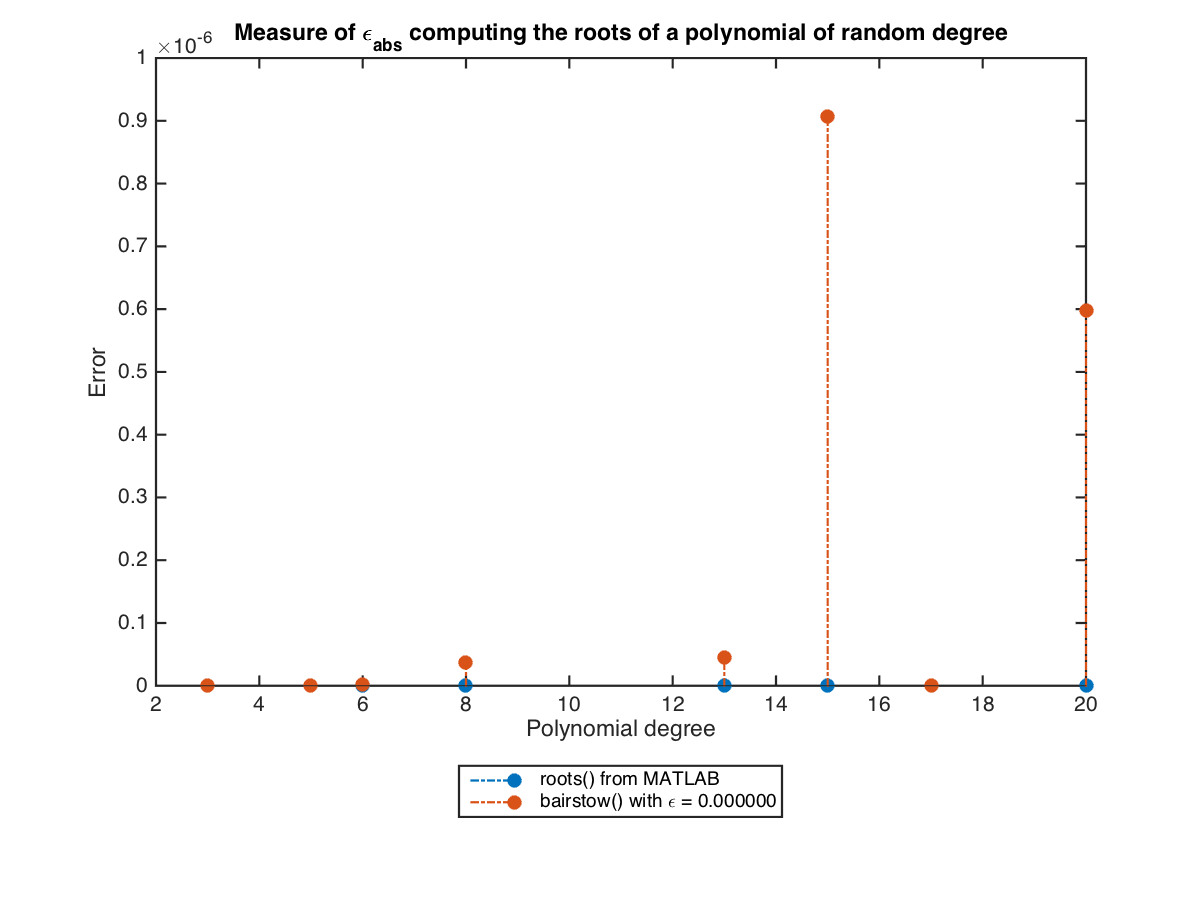
\includegraphics[width=13cm]{data/img/eps6}
    \caption{Cálculo con $\epsilon$ = 0.00000001}
    \label{fig:eps6}
\end{figure}

\begin{figure}[h]
    \centering
    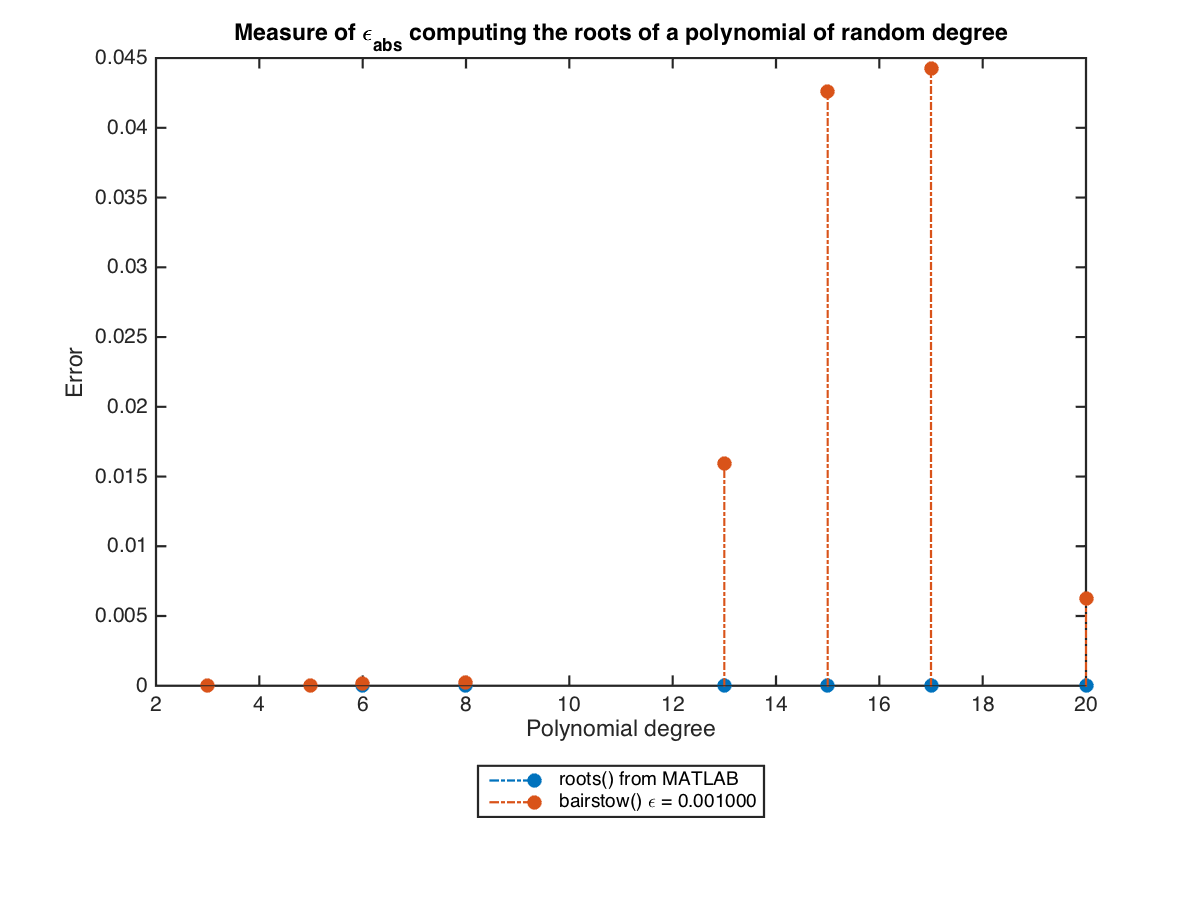
\includegraphics[width=15cm]{data/img/eps2}
    \caption{Medida el error absoluto para el cálculo de las raíces de un polinomio aleatorio dado su grado. Cada medida, corresponde a la suma de las distancias de cada raíz al cero, es decir, el valor real de la evaluación del polinomio en una raíz. Esto, para cada método. Para la ejecución del script \texttt{nroots}, se usó una tolerancia de 0.001, este determina completamente el error obtenido, por lo que se afina este con el objetivo de reducir el error absoluto (Ver figura \ref{fig:eps6}). }
    \label{fig:eps2}
\end{figure}

\newpage

Como puede verse, las limitaciones de la máquina, del lenguaje y del algoritmo, inducen a la presencia de error en el calculo de las raíces de un polinomio, sin embargo, este error aunque no siempre mejor que el de la función nativa, el error es bajo, y puede considerarse un método estable para valores relativamente pequeños de grados de polinomios .

\end{itemize}

%==================================================================

\newpage
\section{Bibliografía}

\begingroup
\renewcommand{\section}[2]{}%
\begin{thebibliography}{}

% Bairstow Bibliography

\bibitem{miller2014numerical} Miller, G. {\em Numerical Analysis for Engineers and Scientists.} 2014. Cambridge University Press. Pags. 175 - 178.

\bibitem{rosloniec2008fundamental} Rosloniec, S. {\em Fundamental Numerical Methods for Electrical Engineering.} 2008. Lecture Notes in Electrical Engineering - Springer Berlin Heidelberg. Pags. 30 - 35.

% Cholesky Bibliography

\bibitem{yang2005applied} Yang, W.Y. and Cao, W. and Chung, T.S. and Morris, J. {\em Applied Numerical Methods Using MATLAB.} 2005. Wiley. Pags. 111 - 112.

\bibitem{suli2003introduction} Suli, E. and Mayers, D.F. {\em An Introduction to Numerical Analysis.} 2003. Cambridge University Press. Pags. 87 - 93.

\bibitem{cheney2007numerical} Cheney, E. and Kincaid, D. {\em Numerical Mathematics and Computing.} 2007. International student edition - Cengage Learning. Pags. 305 - 306.

\bibitem{gander2014scientific} Gander, W. and Gander, M.J. and Kwok, F. {\em Scientific Computing - An Introduction using Maple and MATLAB.} 2014. Texts in Computational Science and Engineering - Springer International Publishing. Pags. 88 - 94.

\bibitem{watkins2004fundamentals} Watkins, D.S. {\em Fundamentals of Matrix Computations.} 2004. Pure and Applied Mathematics: A Wiley Series of Texts, Monographs and Tracts - Wiley. Pags. 32 - 48.

\bibitem{ford2014numerical} Ford, W. {\em Numerical Linear Algebra with Applications: Using MATLAB.} 2014. Elsevier Science. Pags. 267 - 280.

\end{thebibliography}
\endgroup

\bibliography{sample}

\end{document}